\documentclass[quiz]{mcs}

\begin{pcomments}
  \pcomment{FP_product_rule_and_independence}
\end{pcomments}

\pkeywords{
  product_rule
  independence
}

%%%%%%%%%%%%%%%%%%%%%%%%%%%%%%%%%%%%%%%%%%%%%%%%%%%%%%%%%%%%%%%%%%%%%
% Problem starts here
%%%%%%%%%%%%%%%%%%%%%%%%%%%%%%%%%%%%%%%%%%%%%%%%%%%%%%%%%%%%%%%%%%%%%

% F11

\begin{problem}
Construct a probability space $S$ such that $S$ contains three events $A$, $B$,
and $C$ with the following properties:

\begin{itemize}
\item The three events satisfy the product rule.
That is, \[\pr{A \cap B \cap C} = \pr{A} \cdot \pr{B} \cdot \pr{C}\]
\item No two out of the three events satisfy the product rule.
\end{itemize}

\hint It may be helpful to draw a venn diagram for $S$ containing the three
events, and then incrementally fill in the probabilities of the disjoint
regions.

\begin{solution}
One possible answer can be constructed as follows: in the venn diagram shown below,

\[\pr{A} = \pr{B} = \pr{C} = x + y\]
\[\pr{A \cap B} = \pr{A \cap C} = \pr{B \cap C} = y\]
\[\pr{A \cap B \cap C} = y\]

\begin{figure}[h]
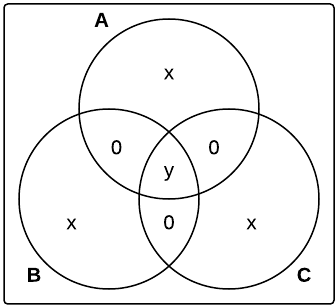
\includegraphics[height=2in]{product-rule-independence-venn.png}
\end{figure}

With this setup, we need to find $x$ and $y$ such that,

\[\pr{A \cap B \cap C} = y = (x+y)^3 = \pr{A} \cdot \pr{B} \cdot \pr{C}\]
\[\pr{A \cap B} = y \neq (x+y)^2 = \pr{A} \cdot \pr{B}\]
\[\pr{A} + \pr{B} + \pr{C} = 3x+y \le 1\]

Take $y = \frac{1}{27}$. From $(x+y)^3 = y$, we get that $x = \frac{8}{27}$.
The second requirement is satisfied since $(x+y)^2 = \frac{1}{9}$, which is
different from $y$. The third requirement is also satisfied since
$3x+y = \frac{25}{27} < 1$.

\end{solution}

\end{problem}

%%%%%%%%%%%%%%%%%%%%%%%%%%%%%%%%%%%%%%%%%%%%%%%%%%%%%%%%%%%%%%%%%%%%%
% Problem ends here
%%%%%%%%%%%%%%%%%%%%%%%%%%%%%%%%%%%%%%%%%%%%%%%%%%%%%%%%%%%%%%%%%%%%%

\endinput
